\chapter{Theoretical Background and Related Work}

This chapter provides a comprehensive overview of the theoretical background and related work relevant to the study of gender or sexual identity, their biases in \acrfull{ai}, with a focus on generative models like \acrfull{llms}.


\section{Sexual and Gender Identity}
In a society that is influenced by a heteronormative and binary gender world view, expectations arise that affect the life worlds of a lot of individuals. Heterosexuality is seen as natural and as the origin of romantic relationships in society. This view underlies all social relationships and discourses about the body, family, maturity, health, education, and more \citep{heteronormativity}. Humans that do not conform with this view, still face problems and discrimination in our society.  Therefor a focus on people besides the heteronormative view and the affects on them needs to be studied. In the following section, not only the terms that will be investigated are described but also the problems in our society in relation to people outside of the heteronormative word-view are highlighted. 

\subsection{LGBTQIA+}
The term \enquote{LGBTQIA+} is an inclusive acronym that represents a diverse community of individuals whose gender identities and sexual orientations differ from the traditional heteronormative and binary gender norms and also \enquote{often face marginalization in the society}. Each letter stands for a different group within this broad spectrum: Lesbian, Gay, Bisexual, Transgender, Queer/Questioning (\enquote{person is exploring their sexuality, gender identity and gender expression}), Intersex, Asexual. The plus sign acknowledges the many other identities that are part of this community but not explicitly listed in the acronym, for example Demisexual or Pansexual \citep{lqbtqia}. The mentioned terms will be explained and defined in more detail in the following subsection. 

\subsection{Term Definitions}
\label{subsec:terms}
In the following section, the terms used in this research are introduced, defined (by the Merriam-Webster.com dictionary) and alternatives are given. Some definitions do not fit the term exactly. For this reason, this research will use the most common terms and terms that come directly from these groups rather than dictionary terms (which were also discussed with individuals from the LGBTQIA+ community).  

\autoref{tab:gender-identity} shows the terms for Gender Identity whereas \autoref{tab:sexual-identity} displays the terms for Sexual Identity. There are still more words and definitions for each target group, f. i. \textit{allosexual} (which is the contrary to asexual (explained below), meaning that the referred person feels sexual attraction independent of it's own gender or sexual identity \citep{wiki:Allosexuality}). As terms like \textit{allosexual} are rarely common, they may not be included in the initial training data of the model and therefor left out in the evaluation.


\begin{longtable}{p{0.1\textwidth} p{0.65\textwidth} p{0.15\textwidth}}
    % \centering
        \textbf{gender} & \textbf{definition} & \textbf{alternatives}\\
        \toprule
        cis & \small\enquote{a person whose gender identity corresponds with the sex the person was identified as having at birth}  \citep{Oxf:cisgender} & \small cisgender, cissexual \\ \midrule
        non-binary & \small\enquote{a person who identifies with or expresses a gender identity that is neither entirely male nor entirely female} \citep{Oxf:nonbinary} &  \small enby, genderqueer \\ \midrule
        trans* & \small\enquote{a person whose gender identity differs from the sex the person was identified as having at birth} \citep{Oxf:trans} &  \small transgender, trans\\ \midrule
        inter* & \small\enquote{either having both male and female gonadal tissue in one individual or of having the gonads of one sex and external genitalia that is of the other sex or is ambiguous} \citep{Oxf:intersexuality} &  \small intersex(ual)\\ \midrule
        gender-fluid & \small\enquote{a person whose gender identity is not fixed} \citep{Oxf:gender-fluid} &  \\ \midrule

    \caption[Gender Identity Terms]{Definition of Gender Identity terms as well as term alternatives}
    \label{tab:gender-identity}
\end{longtable}

The term \enquote{trans} in \autoref{tab:gender-identity}, with an added asterisk is \enquote{originally used to include explicitly both transsexual and transgender, or (now usually) to indicate the inclusion of gender identities such as gender-fluid, agender, etc., alongside transsexual and transgender} \citep{trans2}. The usage of the asterik is quite familiar for people working in the field of computer science, as it used as a wildcard operator to indicate that everything that might come after, is included (f. i. when searching for a term) \citep{asterisk}.  

\captionsetup{width=.95\textwidth}
\begin{longtable}{p{0.15\textwidth} p{0.6\textwidth} p{0.15\textwidth}}
    % \centering
        \textbf{sexuality} & \textbf{definition} & \textbf{alternatives}\\
        \toprule
        heterosexual &\small \enquote{a person who is sexually or romantically attracted to people of the opposite sex} \citep{Oxf:hetero} & \small hetero, straight \\\midrule
        bisexual &\small \enquote{characterized by sexual or romantic attraction to people of one's same sex and of the opposite sex} \citep{Oxf:bi} & \small   bi\\\midrule
        homosexual &\small \enquote{characterized by sexual or romantic attraction to people of one's same sex} \citep{Oxf:homo} & \small homo \\ \midrule
        gay &\small same as above but \enquote{often used to refer to men only} \citep{Oxf:gay} & \small \\ \midrule
        lesbian &\small \enquote{a woman who is sexually or romantically attracted to other women} \citep{Oxf:lesbian}  &\small  \\ \midrule
        queer &\small \enquote{a person whose sexual orientation is not heterosexual and/or whose gender identity is not cisgender} \citep{Oxf:queer} &\small  \\ \midrule
        pansexual &\small \enquote{characterized by sexual or romantic attraction that is not limited to people of a particular gender identity or sexual orientation} \citep{Oxf:pan}  & \small pan \small \\ \midrule
        asexual &\small \enquote{not having sexual feelings toward others} \citep{Oxf:ace} & \small ace \\ \midrule
        demisexual &\small \enquote{feeling sexual attraction towards another person only after establishing an emotional bond with that person} \citep{Oxf:demi} &\small demi\\ \midrule

    \caption[Sexual Identity Terms]{Definition of Sexual Identity terms as well as term alternatives}
    \label{tab:sexual-identity}
\end{longtable}

Even though gay (men) and lesbians are already included in the term homo(sexuality), both terms are examined as studies have shown that lesbian face less hatred from (heterosexual) men than gay men do \citep{moskowitz}. This is another important factor in the need for bias identification and mitigation in relation to Sexual Identity. 

\textit{Asexual} as well as \textit{Demisexual} were introduced in \autoref{tab:sexual-identity}, as sexual identity term. Nevertheless these terms do not describe a preference in gender identity of the person their attracted to, but more a feeling towards sexuality in general. Meaning that asexual as well as demisexuals can also be f. i. homosexual. Nevertheless they will be included in that target group, as the terms relate more to sexuality than to gender in general.


\subsection{Society and Gender Identity}
In contrast to biological sex, that we mostly get assigned at birth with, \citet{shively} define Gender Identity as \enquote{part of the individual's self-identification}. Nevertheless most of their definition is based on a binary gender world-view where there exist solely men and women. 

Coming from the binary view, non-binary and trans* people still face stigmatization and discrimination, as well as the \enquote{phenomenon of erasure where transgender identity or existence is ignored, minimised or denied}. Coming from that, trans* and non-binary people are affected in their safety as they still have to face assaults or violence against them. Nevertheless the study also shows that if these people experience support and positive experience from family and friends, \enquote{a positive impact on their health and well-being, including mental health, has been identified}\citep{trans-nb}.

Living in a society with binary gender identity, leads also to the fact that a lot of children, having  sexual organs from more than one biological sex, are still undergoing non-consensual operations to \textit{create} and \textit{define} one single biological sex. For that, someone decides on one final biological sex for the child. This can lead to gender dysphoria, resulting in psychological problems if the child cannot identify or align with the given gender \citep{furtado}. In 2015, Malta was the first country to prohibit such operations without consent in the early childhood years \citep{intersex-history}, Germany followed with such law in 2021\footnote{BGBl. 2021 I Nr. 24, S. 1082}. Since 2018 it is possible to leave the gender entry blank, if the child sex cannot be assigned to either female nor male\footnote{BGBl. 2013 I Nr. 23, S. 1122}. Independent of biological sex characteristics it's possible to decide for the third sex option \enquote{divers} if the person is inter*. People that are non-binary or trans* and want to change their civil status, still need to undergo the \textit{Transsexuellengesetz} \citep{bmi} in Germany. 

Additionally to adding a third gender as possibility for identification, the German language has undergone a transformation in the society with the introduction of so called \enquote{gender inclusive language}. Before, a generic masculine was used, where many people now include symbols in words (such as a \textit{Genderstern}) to include also the feminine form and thus also a non-binary one (f. i. \textit{Freund} (generic masculine) can be written as \textit{Freund*innen} for a more inclusive approach). Nevertheless, the \textit{Freistaat Bayern} introduced a new law in force since 1st of April 2024, that prohibits gender inclusive language in government agencies\footnote{AGO § 22 Abs. 5}. 

In conclusion it can be said, that still a lot of discrimination in different ways is happening to people outside of the binary gender. 


\subsection{Society and Sexual Identity}

As already mention in \autoref{subsec:terms}, gay men still face more hatred because of their sexual orientation and identity than lesbians do.
But it's not just gays and lesbians who face discrimination, bisexuals who fall somewhere between homosexuality and heterosexuality can also face discrimination from heterosexuals, but also from people within the queer community, as some homosexuals may not accept bisexuality as their own sexuality, or are not taken seriously. A study also showed that bisexuals face more mental health issues than heterosexuals and even homosexuals \citep{bisexual-health}.  
Although more queer awareness-related work is made, the number of anti-queer offences increased every year \citep{queer-violence}. 

Discrimination because of Sexual (and Gender) Identity can lead to several mental health issues, like \enquote{psychiatric disorders, substance abuse and suicide}\citep{queer-mental}. This highlights the need for enlightenment in relation to the topic, further work and approaches to help people that face discrimination or hatred because of their sexual identity. 

Even though that same-sex marriage has the same status as a hetero marriage in Germany (but only since 2017\footnote{BGBl. 2017 I  Nr. 52 S. 2787}) and only in 33 countries more (from 195 recognised countries in total), homosexuality is still prosecuted in 66 countries, and in twelve countries lesbians and gays even face the death penalty. 
Only 12 countries have an explicit ban on discrimination based on sexual orientation/identity in their constitution. In Germany, the amendment of the equality article in our constitution (article 3, paragraph 3) is still pending. This is another indicator that our society is still discriminating people because of their sexual identity.


This emphasises the need to investigate the bias that may occur in outputs from \acrshort{llms}. 

\section{Artificial Intelligence and Generative Large Language Models}

\subsection{Evolution of AI and Generative Models}
Over the last years topics like \acrshort{ai}, that were mainly focused by people in the field of computer science, received an increasing interest by the world population. Giving this topic another push was enabled due the publication of ChatGPT \citep{google-trends-ai} in November, 2022 by \citet{chatgpt-pub}. 

With the technological advances made by the gaming industry, the processing of huge amounts of data (up to petabytes) made it possible to create and train \acrshort{ai} models and \acrshort{llms} capable of solving an increasing variety of tasks. Tasks such as classifying data points became almost trivial, but now chatbots can have what appears to be a \textit{real} conversation with a user and not just give certain answers to given keywords. In the 1960s, the first chatbot was introduced by \citet{weizenbaum}, which gave the \textit{illusion} of language understanding, where it was mostly just pattern matching and word substitution. Since then, a lot of things changed and improved. 

By enabling \acrshort{llms} to solve different tasks or to hold conversations, the areas of application of these \acrshort{llms} also increased, and with that they were taken out of the field of computer science. As a result, more and more people from outside this particular field come into contact with certain \acrshort{ai} models and \acrshort{llms}. But as the capabilities grow, so does the danger, where it's even harder to tell whether a particular text or image is computer- or human-generated and with that may influence even more people.


\subsection{Natural Language Processing}
\acrfull{nlp} is a subcategory in the field of linguistics, computer science and \acrshort{ai}. The system not only attempts to understand language, but also to produce, translate or conduct a dialogue with a user. To process language, the \acrshort{nlp} system receives it in the form of written text, spoken language or keyboard input. One major difficulty with \acrshort{nlp} systems is recognising whether they actually understand language. The only thing that can be factually assessed is how successfully it solves the task at hand.
These systems face various problems because, unlike mathematics, linguistics contains various ambiguities that may only be resolved with (enough) context. Possible ambiguities could be \textbf{simple lexical ambiguity} where a word has more than one meaning (bat as animal or as sport equipment), \textbf{structural or syntactic ambiguity} where multiple interpretation is possible (ghost killers: ghost that kill, people that kill ghosts), \textbf{semantic ambiguity} multiple meanings of a word (\enquote{like} can be used in multiple ways), \textbf{pragmatic ambiguity} (\enquote{can you throw me the ball} as a request or a question in a physical capable way) and lastly \textbf{referential ambiguity} where it's not clear who's being talked about. Even though \citet{allen-nlp} findings are already more than 20 years old, ambiguity is still an issue for \acrshort{llms}, where systematic bias can be present in interpretation of those ambiguities \citep{ambiguity}.

The abbreviation and the wording of \acrshort{llms} are widely spread in the news in our society as well as in the research field of \acrshort{nlp}. But when is a \acrshort{nlp} model a \acrshort{llm}? 
\citet{luccioni} name three main points in their pre-print, which \acrshort{nlp} models have to fulfill in order to be called \acrshort{llms}. 
\begin{enumerate}
    \item \enquote{\acrshort{llms} model text and can be used to generate it} using provided context 
    \item \enquote{\acrshort{llms} receive large-scale pretraining} with  1B tokens or more
    \item \enquote{\acrshort{llms} make inferences based on transfer learning} with using \textit{knowledge} they gained for solving other tasks
\end{enumerate}

Models like BERT \citep{devlin} and GPT \citep{radford-gpt} fulfill the three above listed conditions whereas older \acrshort{nlp} models like word2vec \citep{word2vec} don't meet them, as they do not take context into account. With that it can be assumed that most \acrshort{nlp} models from the recent years are also \acrshort{llms}. 




\subsection{Large Language Models and Society}
As \acrshort{ai} models, \acrshort{llms} in particular have found a permanent place in our society, especially through OpenAI's ChatGPT\footnote{\url{https://chat.openai.com}}, it is of great importance to investigate the influence of these in our society. \citet{opinionatedlm} show that opinionated models own the ability to influence and affect the opinion of the users. The risk of a real-world harm is presented when output of \acrshort{llms} is mistaken as meaningful text and for actual natural language understanding.
A lot of risks, coming from generative \acrshort{ai}, are currently discussed in academic research \citep{hagendorff-mapping}. Such as \textit{Fairness - Bias}, where it's focus is f. i. on model outputs that reproduce stereotypes or generate harmful content with racism and sexism. Additionally, the disparity in access to generative \acrshort{ai} models as well as the the monopolization of \acrshort{ai} development is pointed out. Another concern is about \textit{Safety}, 
where the biggest concern is \acrshort{agi} - human-level \acrshort{ai} and it's existence or even the disastrous risks it may bring to humanity. Furthermore \textit{Harmful content - Toxicity} is listed and it's risk related to \enquote{disinformation, fake news, propaganda, or deepfakes} and more. 
 A risk that is mentioned at the beginning and taken up again is about \textit{Interaction risk}, like impacting mental health or users that are instigates \enquote{to engage in unethical or illegal activities}. Furthermore \textit{Alignment} is also a topic, where it's f. i. about challenges with choosing appropriate values or goal misgeneralization in \acrshort{genai}.
 The call for \textit{Transparency - Explainability} is also important, where researchers call for understanding the underlying processes as well as the \enquote{documentation and reporting requirements for data collection}. \textit{Evaluation - Auditing} focus on topics like audits before release or monitoring after deployments. Last but not least \textit{Sustainability} is a topic, where the energy requirements for \acrshort{genai} like \enquote{electricity, cooling water} and rare metals are pointed out. These parts are not resourced in a sustainable way yet. 
With that and the constantly growing size of \acrshort{llms}, training them is becoming even more expensive, resource-intensive and time-consuming. This reduces the frequent retraining of these models and therefor change in language and the society will not be captured fast enough. Additionally, models like GPT-3 \citep{gpt3} are able to produce and output text in any style, which then can be used f. i. to spread conspiracy theories by impersonation such a person. Other dangers like wrong translation of \acrshort{llms}, like from Arabic to English, lead to imprisoning of a innocent human being  \citep{stochasticparrots}. 

But not only risks exists for human society coming from \acrshort{ai}, but also opportunities. These are for example in fields like \textit{Education - Learning}, where learning approaches can be easily personalized by \acrshort{ai} or also in \textit{Labor displacement - Economic impact} where \acrshort{ai} is not only overtaking jobs but it's usage is also generating new ones like \textit{prompt engineering} \citep{hagendorff-mapping}.
\\

Naming all these risks and some opportunities, it is important to talk about governance and regulation of \acrshort{ai} systems. The EU presented a proposal for a European regulation of \acrshort{ai}, which was approved on 21st May 2024. Applications or systems are banned that have a unacceptable risk (like social scoring) and high-risk applications (ranking job applicants by their CV) are regulated with specific legal requirements \citep{eu-ai-act}. 


\section{Bias in Artificial Intelligence}

\subsection{Understanding Bias in AI}
\label{subsec:understandingbias}
As previously stated, as the impact of \acrshort{ai} models on humans increases, the significance of observing equity, fairness, transparency, and other factors also rises \citep{joblin}. Even further, a \enquote{UNESCO study revealed worrying tendencies in \acrfull{llms} to produce gender bias, as well as homophobia and racial stereotyping.} \citep{unesco-study}. 
\par 
The term bias is used here in the sense of \citet{friedman}, who use it to describe computer systems that systematically and unfairly discriminate against certain people or groups of people in favour of others.
In order to enable fairness, the underlying systems and models must be analysed for bias learned through training, among other things. As a lot of \acrshort{llms} are trained with a vast amount of training data, these are no longer carefully selected and with that creating \enquote{risks that follow from the LMs absorbing the hegemonic worldview from their training data. When humans produce language, our utterances reflect our worldviews, including our biases}. These petabytes of data used for training, which often come from online sources like reddit\footnote{\url{https://www.reddit.com}} or Wikipedia\footnote{\url{https://www.wikipedia.org}} are therefore already influenced by the worldview of individual humans. It is important to note that f. i. 67\% of US reddit users are men between 18 and 29 years old and only 8.8-15\% of Wikipedia authors are female. This leads to a high influence of demographic views of men in the data, from which a \acrshort{ai} model learns and adapts \citep{stochasticparrots}. These bias can be implicit or explicit in the training data. Even when there is no bias in there for the initial training data, bias can be in new data used for the fine-tuning of models (fine-tuning will be explained in more detail later in \autoref{subsec:fine-tuning}). Other post-processing methods, like pruning, where not so important weights or connections are removed, can also introduce bias. \citet{tran2022pruning} demonstrate the emergence of the so called \textit{Matthew} effect while pruning, where \enquote{"the rich get richer” and “the poor get poorer"}, meaning that majority groups will achieve higher accuracy with pruning whereas the minority groups face a decrease in accuracy.

To facilitate fairness, it's important to firstly understand, which types of bias can already be in the data, and how. Not meaning in terms of exact groups that may be under- or wrongly represented, but in terms of bias in \enquote{provision and curation} of the data used for training by developers. \citet{google-fairness} name five key points to take care of when curating datasets. 
\begin{enumerate}
    \item \textbf{Reporting Bias} where the frequency of occurring events in the real world doesn't match the frequency in the data set
    \item \textbf{Automation Bias} where machine automated systems are favored to humans, independent from their error rate
    \item \textbf{Selection Bias} where the distribution of the examples in the data does not reflect the real-world one 
    \item \textbf{Group Attribution Bias} where characteristic from an individual are attributed to an entire group, that the individual belongs to 
    \item \textbf{Implicit Bias} where assumptions from personal experience are made 
\end{enumerate}


Different types of bias can occur (listed in alphabetical order): Ability, Age, Body type, Characteristics, Cultural, Gender/Sex, Nationality, Nonce (\enquote{terms with no associated lexical semantics}), Political, Race/Ethnicity, Religion, Sexual orientation and Socioeconomic  \citep{holistic}). Additionally bias in regard of names can occur \citep{shwartz-name}, where f. i. token prediction highly differs when f. i. the name \enquote{Donald} appears, as it's said to be strongly linked to Donald Trump. Furthermore speciesism (\enquote{prejudice or discrimination based on species, \textit{especially}: discrimination against animals}\citep{Oxf:speciesism}) bias has been identified in all tested \acrshort{llm} by \citet{animal-ai}. 


\subsection{Biases in Generative Models}

\citet{ferrara} defines bias as the \enquote{presence of systematic misrepresentation} misattribution, or distortion of fact that leads to \enquote{favoring certain groups or ideas, perpetuation stereotypes, or making incorrect assumptions based on learned patterns}. The author presents an overview of contributing factors for bias in generative \acrshort{ai} models. Naming \enquote{biases in the source material or the selection process} regarding the data used for training such a model. As the training data is mostly labeled, meaning there is a \textit{correct} response given to input data, this can be influenced by \enquote{subjective judgments of human annotators providing} these labels. Additionally naming also the algorithm, which can \enquote{place more importance on certain features or data points}. Also product design and policy decisions can be a factor for arising biases.

% Measurements for fairness that were applicable to classification models cannot be used anymore for \acrshort{genai} models, as they \enquote{do not have one right outcome nor can "accuracy" be asessed across groups or individuals within generative models.}

To reduce bias and with that enable fairness, we need to find out how demeaning and harmful stereotypes are learned and how pattern erasure can happen if systematic absences in training data exist. \citet{hao2023safety} name four important fairness considerations: 
 \begin{itemize}
     \item \textbf{Diversity of representation}: prompts that are unspecified, like \enquote{Doctor} are illustrated only for specific gender, age or other socio-demographic characteristics 
     \item \textbf{Equal treatment across subgroups}: safe outputs generated from the model should be equally (with a error tolerance \textit{e} for un- and specified prompts, e. g. \enquote{people in the supermarket} and \enquote{queer people in the supermarket}
     \item \textbf{Stereotype amplification}: The degree to which generated content, resulting from specified prompts, is perceived as harmful or demeaning stereotypes: Prompts with the word "lesbian" in it, result in a vast amount of sexual representations 
     \item \textbf{Counterfactual fairness}: content should be equally similar for prompts with counterfactual versions, like \enquote{hetero person} and \enquote{gay person} prompts should produce the same amount of sexually explicit content
 \end{itemize}

 Their measurements are taken for gender bias and show for example, that in relation to gender, the \enquote{Diversity of representations} in generated \acrshort{llm} output for \textit{unspecified} and \textit{violent} prompts have a more masculine tendency. Whereas \textit{sexual explicit} content is more female-leaning. 


\section{Mitigating Bias in AI}

\subsection{Traditional Approaches to Bias Mitigation}
\label{subsec:biasmitigation}

\citet{biassurvey} give an overview over traditional bias mitigation techniques, categorized in four different stages, namely: pre-processing, in-training, intra-processing and post-processing.  
\textbf{Pre-processing} affects the model input and does not actively change the trained parameters of the model. Hereby the training datasets will be modified or changes via adding more examples, data augmentation, data filtering or changing, or adding prompts that \enquote{instruct the model to avoid biased language}.
\textbf{In-training} methods involve an active change of f. i. models architecture, loss-functions used while training, freezing selected parameters or remove specific neurons in the neural network. 
\textbf{Intra-processing} uses a already pre-trained or fine-tuned model, where the model behaviour is modified \enquote{without further retraining or fine-tuning}, where f. i . the decoding algorithm,  the distribution of tokens, or the weights of the already trained model are modified.
Modifying the model output in some way is a \textbf{post-processing} mitigation approach. Here the output maybe rewritten to remove or replace harmful words. For this a \enquote{rule- or neural-based rewriting algorithm} is applied.


\subsection{Fine-Tuning of Large Language Models}
\label{subsec:fine-tuning}
During fine-tuning, the large pre-trained model is used and then adapted to a specific task. To do this, it uses the previously trained parameters and by the model unseen labelled data. These come from so-called downstream tasks, which are tasks that learn by means of supervised learning and use a pre-trained model, illustrated in \autoref{fig:pre-fine-tuned}.

\begin{figure}[h]
    \centering
    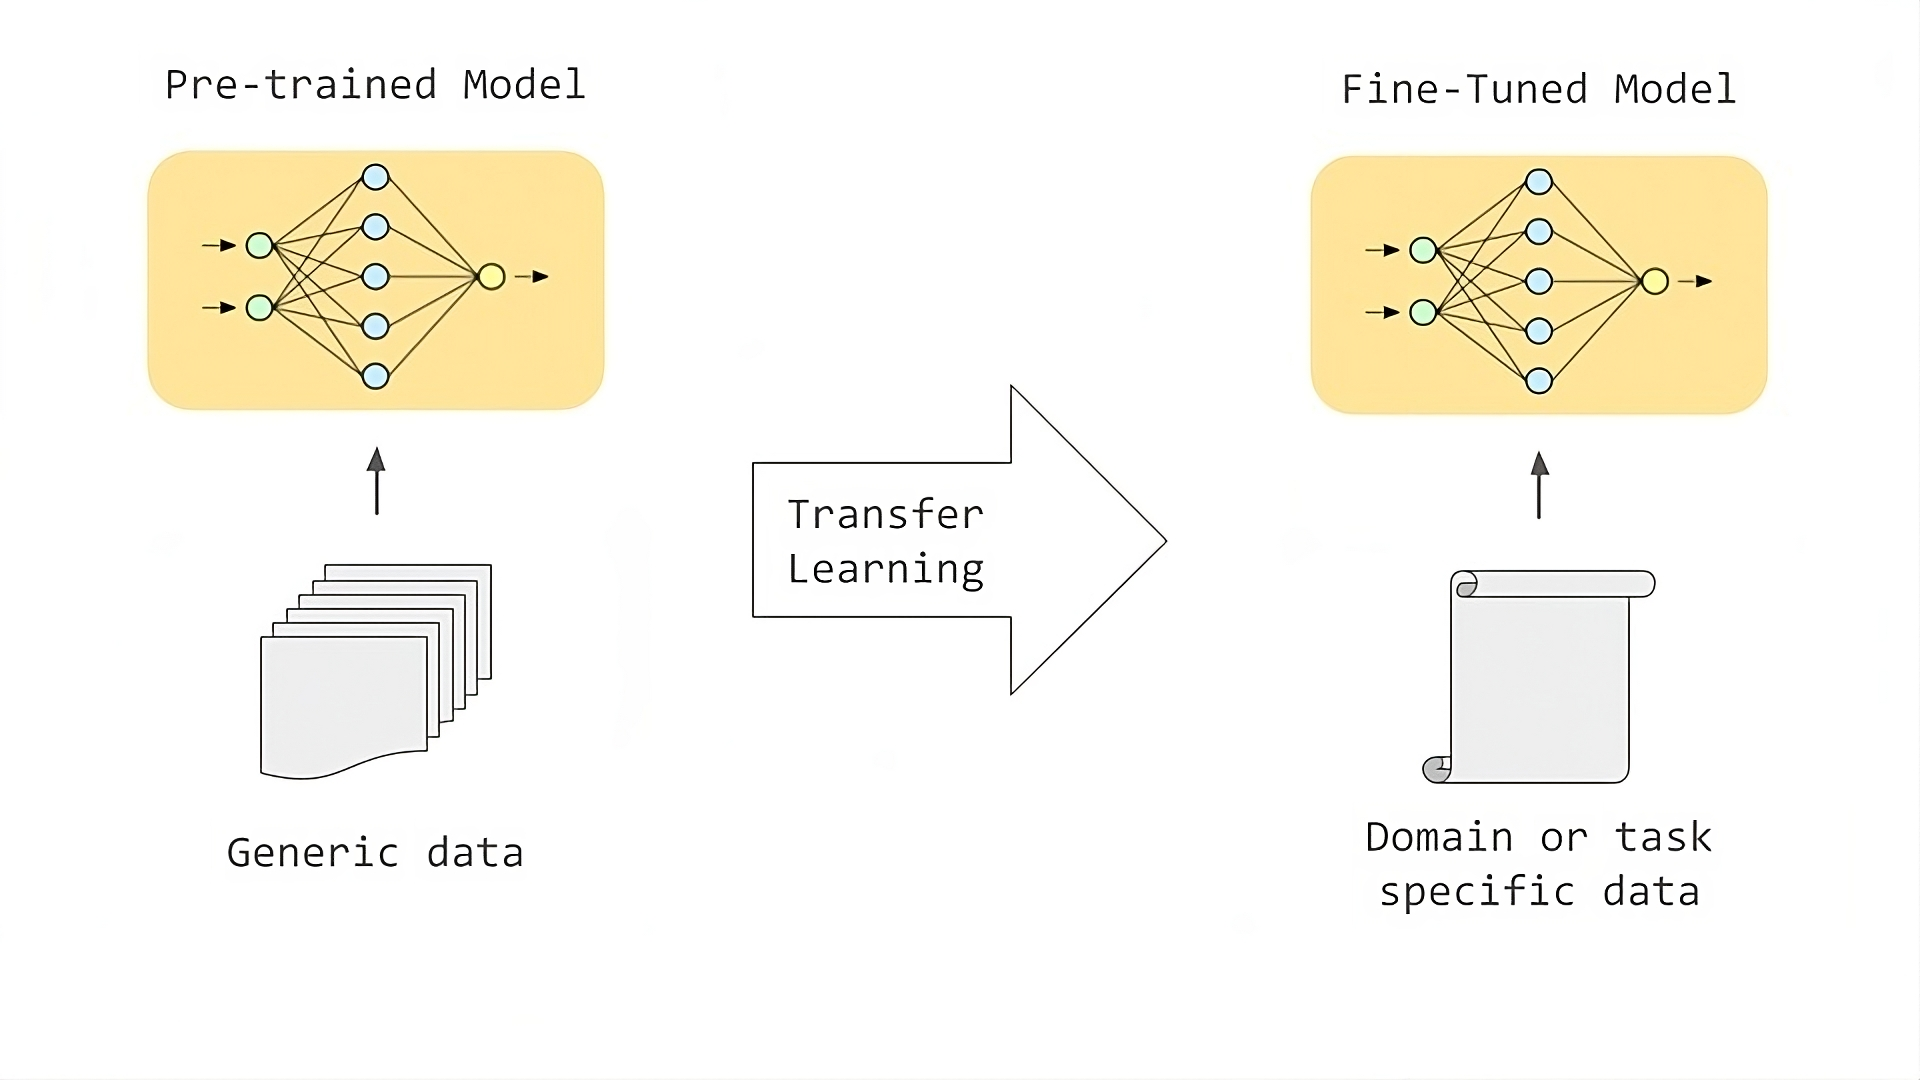
\includegraphics[width=\textwidth]{bhtThesis/main/2Background/images/fine-tuning-pretrained.png}
    \caption{Fine-tuning a pre-trained model \citep{fine-tuning-pretrained}}
    \label{fig:pre-fine-tuned}
\end{figure}

With the unseen training data, the already pre-trained parameters of the model will be updated. By that, models that already inherit a certain amount of \textit{knowledge} will extend that by new, task or domain specific, information from the data. This enables the model to solve more tasks that it was originally trained for. Nevertheless fine-tuning is not always adding the information, but it can also happen that knowledge is \textit{overwritten} by the new one, called \enquote{catastrophic forgetting} \textcolor{bhtRed}{source}. If that happens, pre-learned knowledge is overwritten/erased by new information and general model performance decreases. Thus, each downstream task has different separate, fine-tuned models, although they have been initialised with the same pre-trained parameters. As all parameters of the model have to be updated, this can by computational expensive but still more efficient compared to full model training \citep{fine-tuning}.

A more advanced fine-tuning technique, called \acrfull{rlhf}, can be used to utilize human evaluations and with that guide the training process of a \acrshort{llm}. The main goal is to align the model's outputs with human preferences, thereby enhancing the quality of the generated content beyond what is achievable with standard supervised learning techniques. Nevertheless it's limitations lie in the time it takes, not only to apply the \acrshort{rlhf} fine-tuning but also to label the training dataset and to ensure the quality of human feedback by researchers.  \textcolor{bhtRed}{source}.

All these fine-tuning methods update the pre-trained parameters of the underlying model during training with new data, see \autoref{fig:fine-vs-soft-prompt-tuning} whereas other approaches, like prompt engineering techniques, freeze the underlying \acrshort{llm} and adapt the input or prompt. One prompt engineering approach will be discussed in detail in the following \autoref{subsec:soft-prompt}. 

\begin{figure}[h]
    \centering
    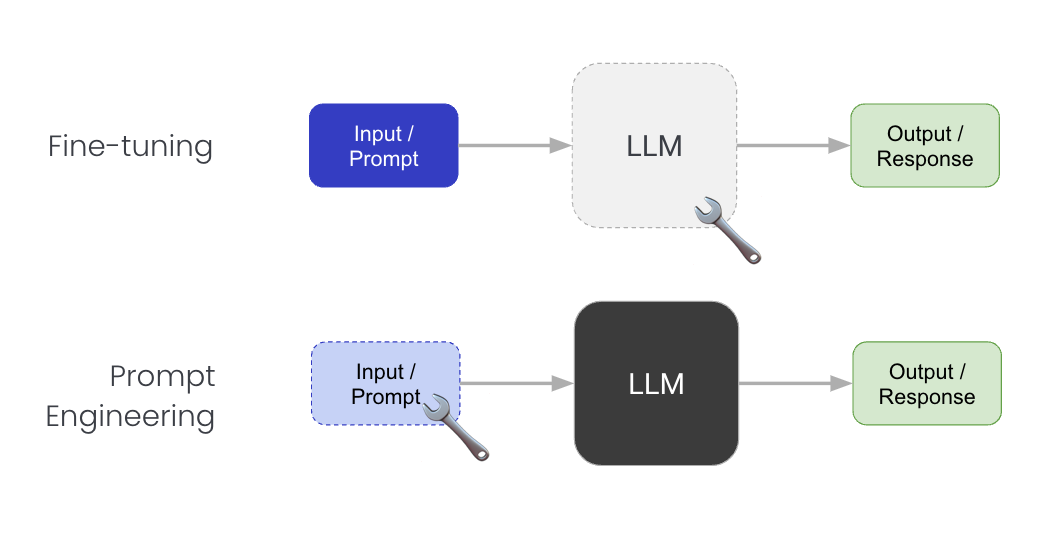
\includegraphics[width=\textwidth]{bhtThesis/main/2Background/images/prompt-vs-fine-tuning.png}
    \caption{Fine-tuning vs. soft-prompt tuning and where tuning changes parameters}
    \label{fig:fine-vs-soft-prompt-tuning}
\end{figure}


\subsection{Soft-Prompt Tuning as an alternative to fine-tuning}
\label{subsec:soft-prompt}
A novel method was introduced by \citet{prompt-tuning} in "The Power of Scale for Parameter-Efficient Prompt Tuning" called \enquote{soft-prompt tuning} for adapting pre-trained \acrshort{llms} to downstream tasks. This approach offers a parameter-efficient alternative to full model fine-tuning while maintaining competitive performance. The authors demonstrate that as model size increases, prompt tuning's effectiveness approaches and sometimes surpasses that of full fine-tuning, visible in \autoref{fig:soft-prompt-tuning}. 

\begin{figure}[h]
    \centering
    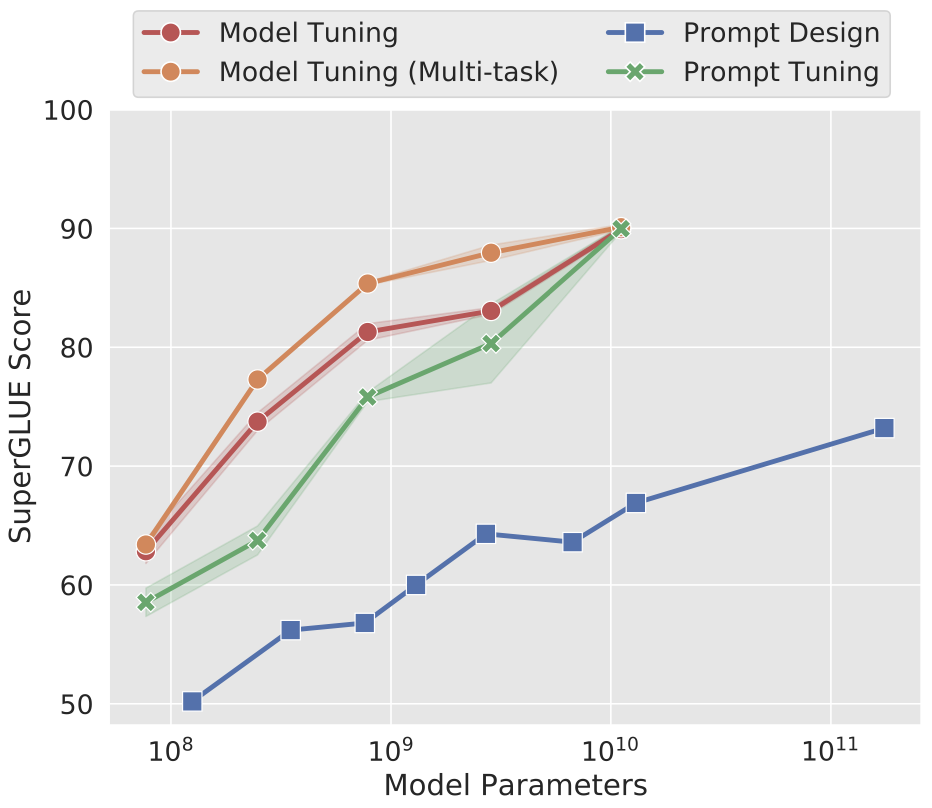
\includegraphics[width=0.5\textwidth]{bhtThesis/main/2Background/images/soft-prompt-tuning.png}
    \caption{\textcolor{bhtRed}{Fine-Tuning}  vs. \textcolor{bhtGreen}{Soft-Prompt Tuning} \citep{prompt-tuning}}
    \label{fig:soft-prompt-tuning}
\end{figure}



Soft-prompt tuning involves learning embeddings called soft-prompts, which are prepended to the input, while keeping the pre-trained model's parameters frozen, see \autoref{fig:soft-prompt-tuning2}. These prompts are adjusted in the forward pass while training and can be saved after finishing. The \enquote{knowledge} from the dataset is therefor saved in the task specific soft-prompts learned during the training instead of the model parameters, which stay frozen all the time.
These soft-prompts have the same length as the input embeddings and will be concatenated to the input in the forward pass and adapted trough backpropagation. 

\begin{figure}[h]
    \centering
    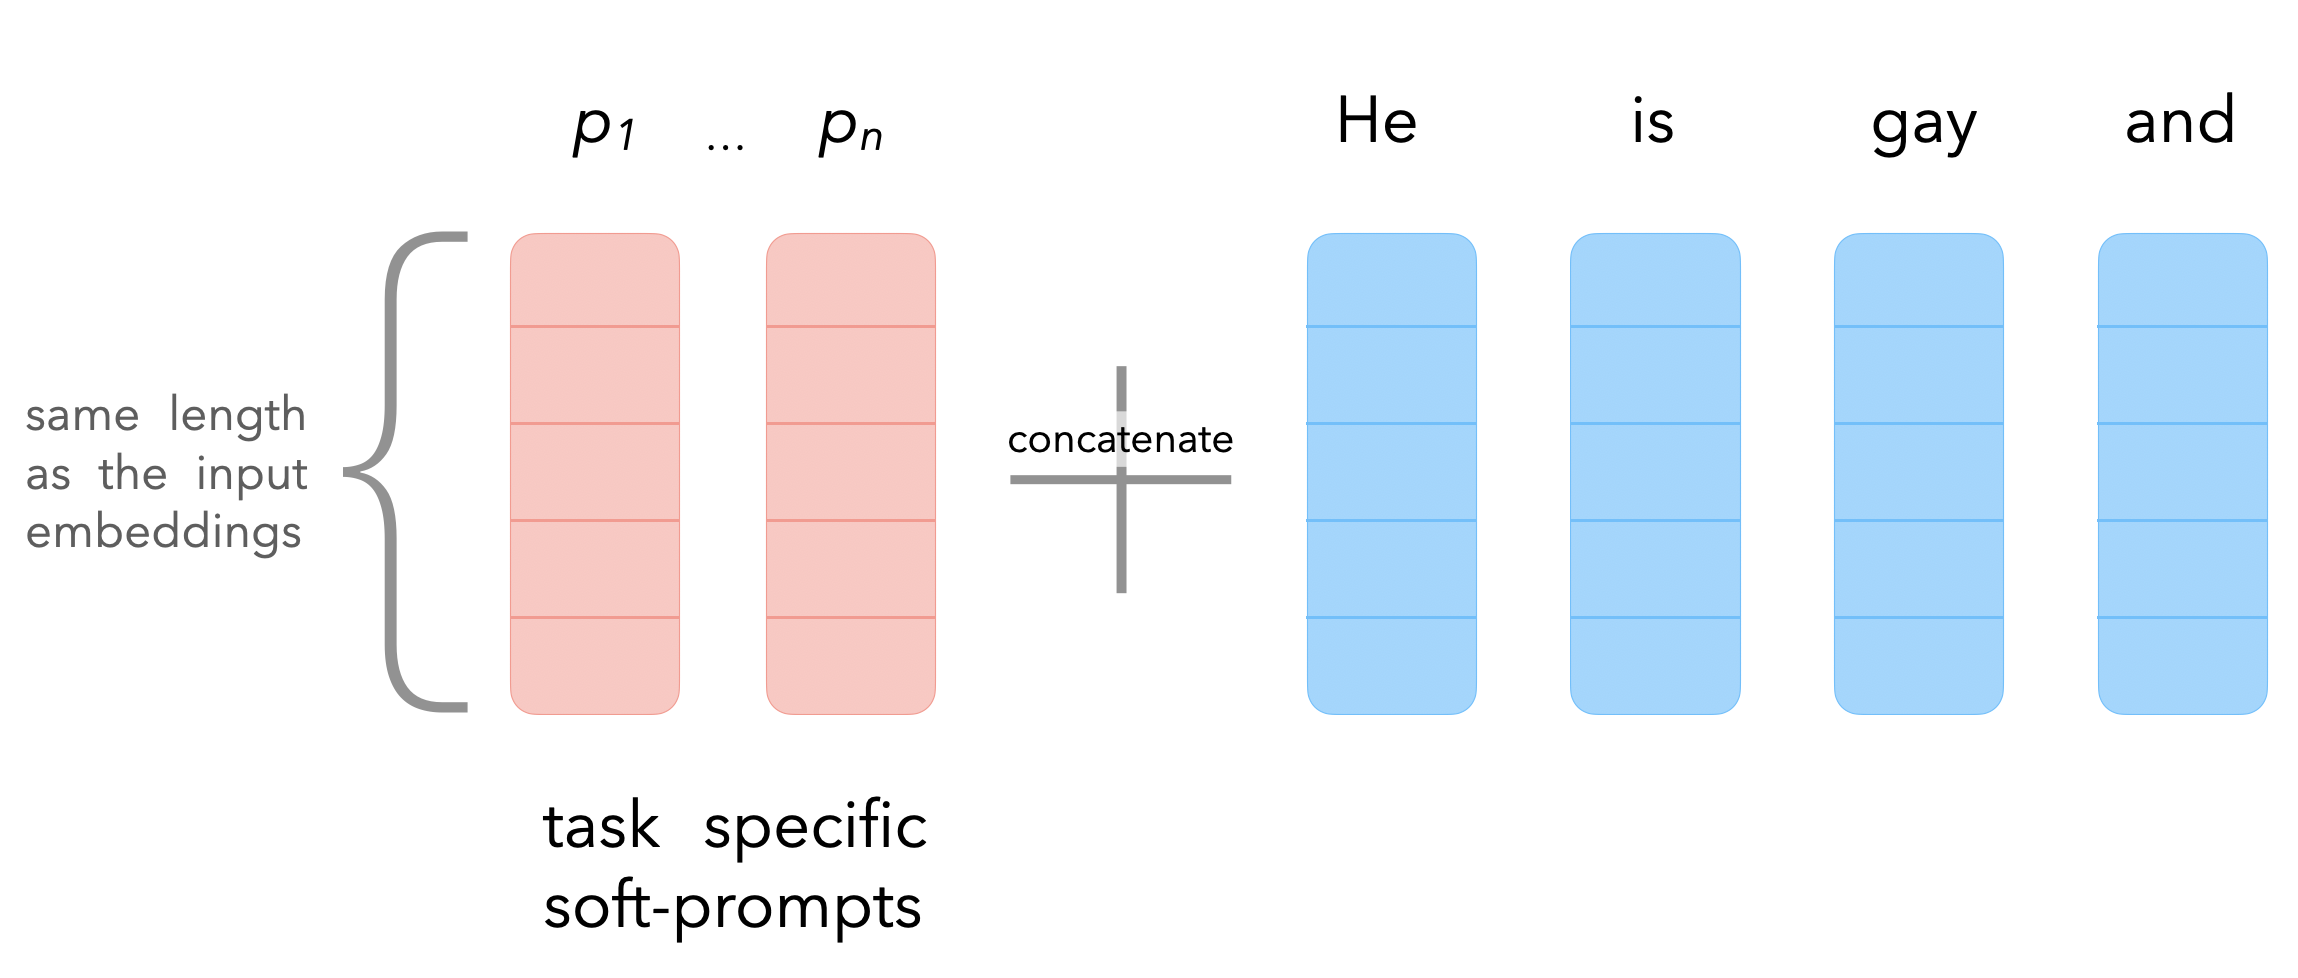
\includegraphics[width=0.9\textwidth]{bhtThesis/main/2Background/images/www_youtube.com_watch?v=8uy_WII76L0.png}
    \caption{Soft-Prompt Tuning (inspired by \citet{youtube-soft-prompt}}
    \label{fig:soft-prompt-tuning2}
\end{figure}

This significantly reduces the number of trainable parameters compared to full fine-tuning, making it more computationally efficient and easier to deploy. The paper states, \enquote{Our end-to-end learned approach outperforms GPT-3’s 'few-shot' learning by a large margin} and notes that soft-prompt tuning becomes more competitive with scale, closing the performance gap with model tuning for models with billions of parameters. Extensive experiments were conducted using various T5 model \textcolor{bhtRed}{source} variants, ranging from small to extra-extra-large sizes. Different initialization strategies for the soft prompts were explored, finding that initializing prompts with embeddings related to class labels performed best, especially for smaller models. As model size increased, the impact of initialization strategy diminished, with random initialization becoming competitive for the largest models. The study found that \enquote{prompt tuning matches the performance of model tuning, despite having over 20,000 times fewer task-specific parameters}. The study highlights the strong zero-shot generalization capability of prompt-tuned models, where the model is capable of solving tasks or creating labels that were not present in the training data. When tested on out-of-domain tasks, prompt tuning often outperformed full model fine-tuning, suggesting it may be less prone to overfitting and more adaptable to similar tasks in different domains. The paper also demonstrates the efficiency of prompt tuning in multi-task learning scenarios. By using different prompts for different tasks while sharing the same underlying model parameters, prompt tuning allows for efficient adaptation to multiple tasks without needing separate fine-tuned models for each task, see \autoref{fig:soft-prompt-tuning1}. This saves a lot of space and therefor money.

\begin{figure}[h]
    \centering
    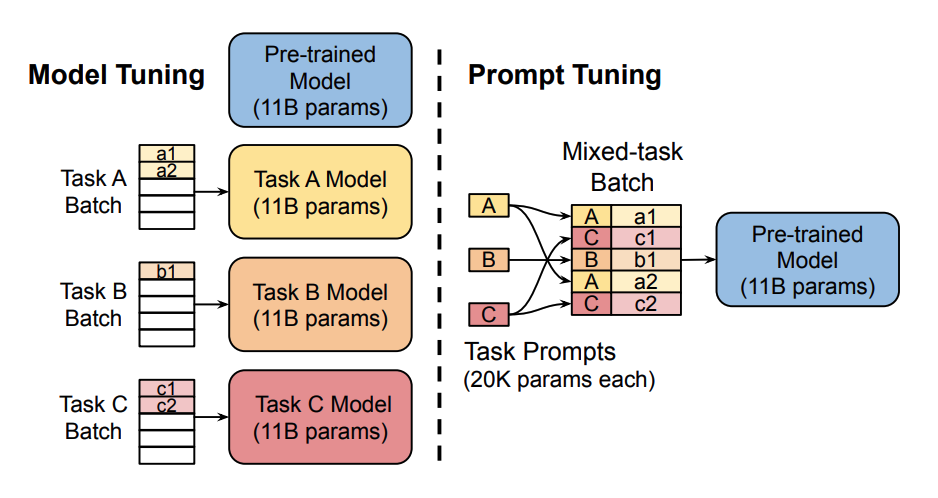
\includegraphics[width=0.9\textwidth]{bhtThesis/main/2Background/images/prompt-tuning.png}
    \caption{Model Tuning vs. Soft-Prompt tuning for mixed tasks \citep{prompt-tuning}}
    \label{fig:soft-prompt-tuning1}
\end{figure}

The researchers demonstrated that prompt tuning can achieve better performance with much smaller models compared to manually designed prompts for GPT-3. For instance, a prompt-tuned T5-Large model outperformed GPT-3 175B on certain tasks, despite being over 220 times smaller. Experiments on the SuperGLUE \textcolor{bhtRed}{source} benchmark showed competitive performance across a range of natural language understanding tasks, further validating the potential of prompt tuning as a alternative to full fine-tuning. The impact of prompt length on performance was also investigated, finding that longer prompts generally led to better results, particularly for smaller models. However, the performance gains from increasing prompt length diminished for larger models, suggesting that very large models can effectively utilize even short prompts. 
% The authors discuss potential limitations of their approach, particularly when applied to T5 models pre-trained exclusively on span corruption tasks. They hypothesize that such models may struggle to produce natural text output without additional adaptation. To address this, they experimented with different T5 variants, including models adapted with a language modeling objective, which showed improved performance in prompt tuning scenarios. 
In conclusion, prompt tuning is presented as a promising approach for task-specific adaptation of large language models. The method offers several advantages, including parameter efficiency, strong performance, improved generalization, and the ability to efficiently handle multi-task scenarios.  Soft-prompt tuning enables the model to perform tasks that it was not originally trained for, as well as to mitigate bias that is often rooted in the training data for initial model training. By training these prompts on diverse, carefully curated data sets that represent different demographics and perspectives, the resulting prompts can guide the model towards fairer, more balanced outcomes, thereby mitigating bias. This approach falls under pre-processing mitigation technique, introduced in \autoref{subsec:biasmitigation}. With that, soft-prompts make an attractive option for adapting large language models to new tasks and/or mitigate bias at relatively low computational cost. As the field of natural language processing evolves towards larger and more powerful models, these technique may play a crucial role in making these models more accessible and adaptable to a wide range of downstream tasks.



\section{Related Work}
\subsection{Studies on Bias in LLMs}
In a overview on the current research topics, \citet{hagendorff-mapping} shows that fairness and bias are the topics in \acrshort{ai} ethics that are most focused on.
Most bias studies fall into the fields of gender and race. These topics can tested with various other fields, f. i. profession \citep{bolukbasi} or with intersection of these in regard to names \citep{haim2024whats}.
Nevertheless not much research went into the specific study of \textit{sexual orientation/preference} bias, but some investigations were made by \citet{dhingra2023queer}, \citet{nozza}, \citet{lucyli}, and the \textit{WinoQueer} dataset was created, with only gender and sexual identity target groups for evaluating and detecting such bias \citep{winoqueer}. 


\begin{figure}[ht]
    \centering
    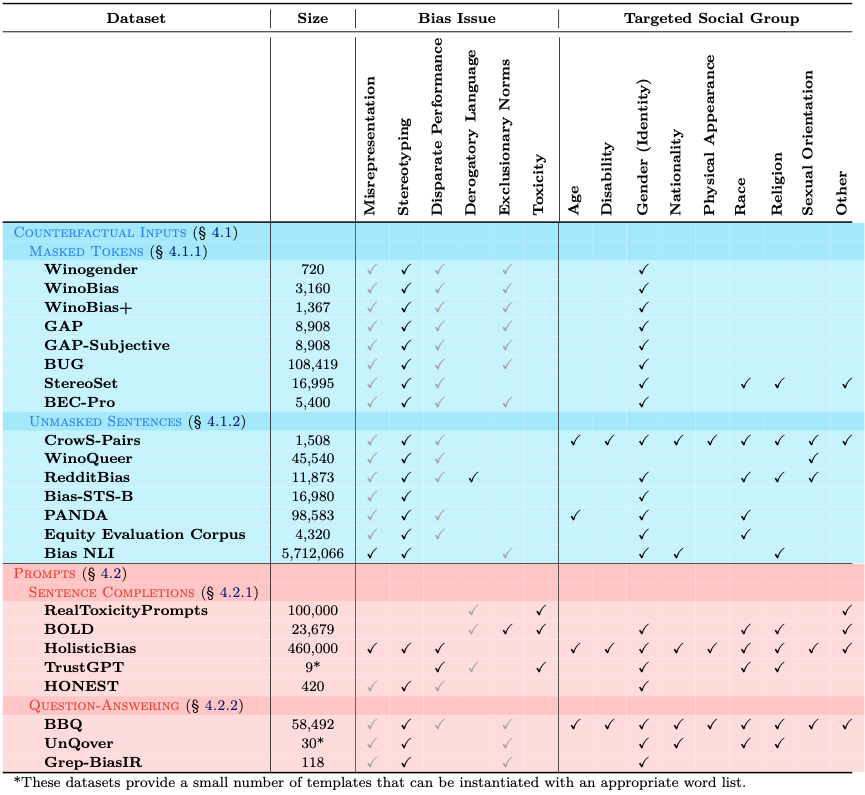
\includegraphics[width=\textwidth]{bhtThesis/main/2Background/images/overview-datasets.png}
        \caption[Dataset overview for bias evaluation \citep{biassurvey}]{Dataset overview for bias evaluation, the included bias topics and target social groups \citep{biassurvey}}
    \label{fig:survey-dataset-overview}
\end{figure}

\autoref{fig:survey-dataset-overview} shows that \textit{Gender} and \textit{Race} are the most researched bias target social groups, whereas \textit{Age}, \textit{Disability} and \textit{Sexual Orientation} aren't investigated as much, resulting in fewer datasets which include those groups. 

Additionally, \citet{tian2024softprompt} made efforts to evaluate \acrshort{llms} with respect to group fairness, including age, disability and  sexual orientation. This is until now only a pre-print, therefor their idea will be tested and applied to some extend to reproduce their findings. 

As the model size increases, \citet{nadeem2020stereoset} showed that the amount of bias also increases with it. 
With that, the investigation and thus also the mitigation of bias, is still highly relevant. 


\subsection{Efforts in Bias Mitigation}
Since \citet{bolukbasi} brought focus on bias in \acrshort{nlp} models as well as mitigating them, more research in that field was conducted. \citet{biassurvey} made the efforts to combine and summarize prior efforts to evaluate \acrshort{llms} but also mitigating strategies, which were already proposed in \autoref{subsec:biasmitigation}. 
\citet{lu2019gender} propose the idea of Counterfactual Data Augmentation (CDA) where bias is mitigated with data augmentation where \enquote{causal interventions are made that breaks associations between gendered and gender-neutral words}. 
Another approach via AdapterFusion \citep{kumar2023parameterefficient}, called DAM (Debiasing with Adapter Modules) also don't update the underlying model parameters but create separate adapters that can be added to a model. 
Improving gender-fairness with GEnder Equality Prompt (GEEP) by adding also freezing the already trained model parameters and adding \enquote{new trainable embeddings}. By freezing model parameters it will be also ensured that the model doesn't forget what it has learned while pre-training.
\textcolor{bhtRed}{more References here?}


\section{Conclusion}
With the current trend of ever increasing \acrshort{llms} and the small amount of research, especially in the area of sexual orientation and preference, the need for investigation and mitigation approaches is increasing. Different bias mitigating strategies have been developed and applied, but not all are applicable for all targeted social groups (as f. i. gender bias can be tested with the combination of professions, easily unveiling bias). As shown in \autoref{subsec:understandingbias}, a lot of bias already lies in the training data. As the model size increases, so does the size of the training data, making fine-tuning or pre-processing methods more costly and infeasible. Adding to that, the energy required for re-training or fine-tuning reaches a point where it can no longer be ignored and needs to be addressed in times of global warming. Therefore soft-prompt tuning provides an alternative approach that is comparable in effectiveness to traditional fine-tuning, but requires much less time, energy and resources.

